To evaluate our approach, we apply it to a real-life event log about a loan application process from a financial institute.
The log is from the BPI Challenge 2012 \cite{bpi2012log} and contains $262,200$ events in $13,087$ cases. It is actually composed of three intertwining subprocesses. Overall, cases start with an application, then multiple offers may be sent back and forth until the application is cancelled, declined or accepted. And in between, there can be work events pertaining to communication between employees and applicants. Since this makes the the process model discovery unfeasible, we focus just on the offer subprocess by projecting the entire log onto the activities starting with \emph{O\_}. This leaves $5015 cases$. It is important to note here, that the log was extracted from a running system and thus contains unfinished cases.
The model in Figure \ref{fig:goodmodel} describes this subprocess very well (fitness of $0.957$). Offers start are first selected, are then created and sent. At this point, they are either sent back, and end up declined or accepted, or are cancelled and either end immediately or loop to the beginning. One deviation is that sometimes, when the loop is taken, the cancellation occurs after the new selection.
\begin{figure}
    \centering
    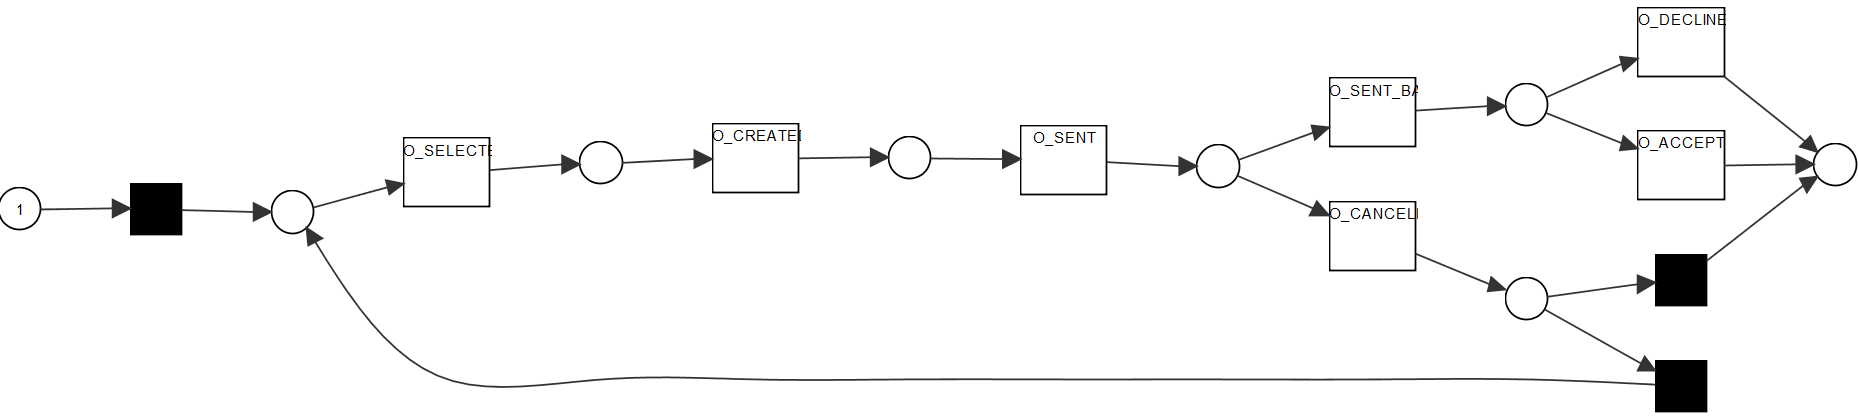
\includegraphics[width=\textwidth]{figures/evaluation/good_model.png}
    \caption{A good model describing the offer subprocess}
    \label{fig:goodmodel}
\end{figure}

We will purposely use an overfitting model which removes this looping possibility to highlight the advantages of our approach.
Applying the state of the art conformance checking plugin \emph{Replay a Log on Petri Net for Conformance Analysis} yields a fitness of $0.88$ and colorization of places based on their involvement in non-sync moves.
%\begin{figure}[H]
%    \centering
%    \includegraphics[width=\textwidth]{figures/evaluation/bad_model_conf.png}
%    \caption{Standard conformance analysis of the overfitting model}
%    \label{fig:badconf}
%\end{figure}
We now apply our plugin to obtain more fine grained results. After computing the alignment, it takes about half a second, to locally map the log. The export of the dataset for one place takes about a minute.
\begin{figure}[H]
    \centering
    \includegraphics[width=\textwidth]{figures/evaluation/bad_model_sink_prob.png}
    \caption{Problem view of the sink place}
    \label{fig:badsinkprob}
\end{figure}

In the problem view of the the last place in Figure \ref{fig:badsinkprob}, we can see that over relative time, there are lots of cancellations without an accompanying trace end right at the start. The result view also tells us, that $51.87\%$ of cancellations were somehow incorrect. We also see that due to this, the fitness timeseries is quite low at the start.
The opposite happens at the source place where the fitness (over relative time) drops to zero almost immediately because only the first execution of \emph{O\_SELECTED} was actually possible in the model. Especially the scatter plot in Figure \ref{fig:badsourcescatter} suggests that there must be a loop in the log.
\begin{figure}[H]
    \centering
    \includegraphics[width=0.6\textwidth]{figures/evaluation/bad_model_source_scatter.png}
    \caption{Scatter plot of interactions of the source place}
    \label{fig:badsourcescatter}
\end{figure}

For the place at the first split between \emph{O\_CANCELLED} and \emph{O\_SENT\_BACK}, we notice a drop in fitness towards the end caused by cancellations without the offer first being sent. This may be caused by the fact that the log contains cut-off traces towards the end of the recorded period.

For performance, \emph{Replay a Log on Petri Net for Conformance/Performance Analysis} colors the places similarly to our plugin based on the average sojourn time. For the aforementioned place, which has the highest impact on case duration, the average sojourn duration given is $12.47$ days with a standard deviation of $9.36$ days. Our average is $10$ days with the a standard deviation of $9$ days. This is because we consider log moves which are abundant in this scenario where in reality multiple loops can occur but the model only supports the first one. With different settings, i.e. ignoring log moves, we can also reproduce the $12$ day measure. We can therefore conclude that later loops are usually shorter. The high standard deviation already hints at an unstable performance but Figure \ref{fig:badsplitperf} shows in more detail that the typical sojourn duration really breaks in towards the end which would be a good thing if it was not for the correlating decrease of fitness and dwindling number of incoming complete interactions ($\func{lbusyness_{c\_int}}$).
\begin{figure}
    \centering
    \includegraphics[width=0.7\textwidth]{figures/evaluation/bad_model_split_perf.png}
    \caption{Performance graph of the place at first split}
    \label{fig:badsplitperf}
\end{figure}

This evaluation showed the advantages of the most prominent features which are the timeseries of metrics. An analysis of the exportable dataset is out of the scope of this evaluation but may lead to even more promising results.